\documentclass[12pt]{article}

% ---- Includerer eksterne filer ------------------------------
\input{metadata.tex}
\input{biblioteker.tex}
\addbibresource{referanser.bib}
\input{includes/forside.tex}
\input{preamble.tex}


% --------------- Dokument -----------------------------
\begin{document}

\makedoctitle

\pagenumbering{Roman}
\setcounter{page}{1}

\tableofcontents

\clearpage
\addcontentsline{toc}{section}{Sammendrag}
\section*{Sammendrag}
I dette prosjektet analyseres lydklippet fra sangen “Seven Nation Army” 
av The White Stripes ved hjelp av Fast Fourier Transform (FFT) og Short-Time 
Fourier Transform (STFT). Målet er å undersøke hvordan Fourier-transformasjoner 
kan brukes til å identifisere og visualisere de dominerende 
frekvenskomponentene i et musikkstykke, samt forstå hvordan disse 
varierer over tid. FFT benyttes for å identifisere hovedfrekvensene og 
harmoniske overtoner i hele signalet, mens STFT muliggjør en tids-frekvensanalyse 
som viser dynamiske endringer i energi og rytmikk.

Analysen viser at de lavfrekvente komponentene mellom 50 - 120 Hz dominerer lydbildet, 
og representerer sangens karakteristiske basslinje. Gjennom spektrogrammet fremkommer 
tydelige mønstre som samsvarer med slagverk og rytmiske elementer i mellomfrekvensområdet 
(500 - 2000 Hz). Resultatene bekrefter at Fourier-transformasjoner gir et presist og 
intuitivt bilde av hvordan både harmoniske og rytmiske strukturer danner grunnlaget for musikken.

Videre drøftes effekten av ulike vindustyper og parametervalg i STFT-analysen. 
Hann-vinduet ble valgt for å balansere mellom tids- og frekvensoppløsning og 
for å redusere spektrallekkasje. Prosjektet viser hvordan matematiske transformasjoner 
kan anvendes i musikkteknologi for å analysere og tolke lydsignaler, og legger 
grunnlaget for videre arbeid med mer avanserte metoder som wavelet-transformasjon 
eller maskinlæringsbasert lydklassifisering.

\clearpage

\pagenumbering{arabic}          % Bytter til vanlige tall fra romertall
\setcounter{page}{1}

\section{Innledning}
\input{includes/innledning.tex}

\clearpage

\section{Teori}
\input{includes/teori.tex}

\clearpage

\section{Metode}
\subsection{Forberedelse av lydfil for analyse}
For å kunne ta i bruk den numeriske løsningen av bølgeligningen, må lydfilen først forberedes. Dette gjøres ved å lese inn lydfilen 
og konvertere den til et format som kan brukes i den numeriske modellen. I dette prosjektet benyttes Python-biblioteket 
\verb|scipy.io.wavfile| for å lese inn lydfilene i WAV-format. Det er blitt valgt å bruke en avgrenset del av lydfilen for å redusere kompleksiteten
i analysen og fokusere på de mest relevante delene av signalet. Dette lar oss også identifisere enkelte toner med STFT-analyse og forhåpentligvis kunne
identifisere instrumentene som produserer disse tonene.

Når det gjelder samplingsrate, ble det brukt den standard samplingsraten på 44100 Hz for lydfilen. Dette er en vanlig samplingsrate for 
lydfiler og gir en god balanse mellom lydkvalitet og filstørrelse. Dette gir en analyserekkevidde opp til 22050 Hz, i henhold til Nyquist-teoremet.
Det også viktig å velge en høy nok samplingsrate for å sikre at de høyeste frekvensene i lydsignalet blir korrekt representert, hvis ikke kan aliasing oppstå.

\subsection{Analyseringsprogram i python}

I dette delkapittelet beskrives koden for å fouriertransformere en sangfil, med fft. Koden kan hentes her: 
\parencite{python_fft_analyse} 

For å analysere lydsignalet til en sang, har programmeringsspråket python blitt brukt, da med
pakkene \texttt{numpy}, \texttt{matplotlib}, og \texttt{scipy}for å animere og plotte grafen. 
Pakkene \texttt{subprocess}, \texttt{progressbar}, og \texttt{argparse} har blitt brukt for 
å kjøre eksterne programmer, se status på rendering av animasjon og hente inn kommandolinjeargumenter når
programmet blir kjørt. 

\subsubsection{Animasjonsfunksjonen}

Først brukes \texttt{scipy} biblioteket sin funksjon \texttt{wavfile.read} for å lese av input filen.
Denne returnerer \texttt{sampleRate}, som er hvor mange ganger per sekund den analoge bølgen for 
sangen har blitt målt. Det andre funksjonen returnerer er \texttt{wav}, som er array fra 
\texttt{numpy} biblioteket. Denne arrayen består av alle samplingene til sangen. Deretter blir
lengden på arrayen lest av for å finne ut hvor mange samplinger det er i sangen. 

Ettersom samples i en wav fil kan bli enten lagret som \texttt{float} (desimaltall) fra 
\texttt{[-1.0 , 1.0]} eller \texttt{int16} (16 bit integer) fra \texttt{[-32768 , 32768]}, brukes det
en \texttt{if}-sjekk for å sørge for at det kun er desimaltall innenfor \texttt{[-32768 , 32768]} 
som brukes for å tegne på grafen. Deretter blir wav-arrayen sjekket for om det er en eller 
to kanaler. Dersom det er to kanaler, blir kanalene lagt sammen til en kanal for å få med seg
alle frekvensene uten å måtte fouriertransformere hver kanal for seg. 

Deretter kommer seksjonen i koden der viktige variabler blir satt. Først defineres \texttt{spf} eller \textit{samples per frame}, 
, som er antall samplinger mer bilde som renderes i animasjonen. Deretter defineres \texttt{T = 1.0 / sampleRate}, som er 
hvor lang tid det er mellom hver sample i wav-filen. Antall samples per fouriertransformasjon defineres av 
\texttt{N = max(2, fftTime * sampleRate)}, der \texttt{fftTime} er ett av funksjonsargumentene, som definerer
hvor langt tidsintervall som skal fouriertransformeres om gangen. For å finne ut hvor mange bilder som skal lages
i videoen, brukes formelen  \texttt{totalFrames = max(o , (len(wav) - N) // spf + 1)}. Stykket finner ut hvor mange samples 
som er med, minus ett vindu, og deretter delt på antall samplinger per bilde. 

For å regne ut hvilke verdier en for langs x-aksen, blir \text{scipy} biblioteket sin \texttt{rfftfreq} funksjon brukt.
\texttt{rfftfreq(N, T)} returnerer en array av positive frekvensverdier, frem til Nyquist-frekvensen som er halvparten
av samplingsraten. \texttt{[: N //2]} gjør at frekvensaksen passer med resultatet for fouriertransformasjon av signalet.

\subsubsection{Fouriertransformasjon per bilde}

Det er funksjonen \texttt{fftWav(n)} som håndterer fouriertransformasjon per bilde i animasjonen. Variablen \texttt{n}
representerer bildenummeret i hele arrayen. Funksjonen starter ved å definere \texttt{n0} og \texttt{n1}, som er rammene
til hvor i wav-arrayen en skal fouriertransformere fra og til. Dette skjer ved å definere \texttt{fftwav = wav[n0:n1]}, 
som kutter \texttt{wav} fra \texttt{n0} til \texttt{n1}. \texttt{n0} blir bestemt ved uttrykket \texttt{n * spf - N // 2},
der den hopper \texttt{n * spf} samplinger frem i wav-arrayen, og trekker fra halvparten av \texttt{N} som startverdi.
Deretter sjekkes det om arrayen som skal fouriertransformeres for bildet er like lang som \texttt{N}. Hvis ikke legges
det til ekstra verdier for å få arrayen til riktig størrelse. Dette betyr at de siste bildene vil ha noe unøyaktig 
fouriertransformasjon. Denne arrayen blir så multiplisert med hanning-vinduet \texttt{window}. Deretter fouriertransformeres arrayen \texttt{fftWav} med \texttt{scipy} sin funksjon \texttt{rfft}.
Den nye arrayen blir kalt \texttt{yf}. Nå kan denne arrayen inneholde negative verdier, derfor må en gjøre disse positive og 
normalisere resultatet. 

\begin{figure}[H]
	\centering
	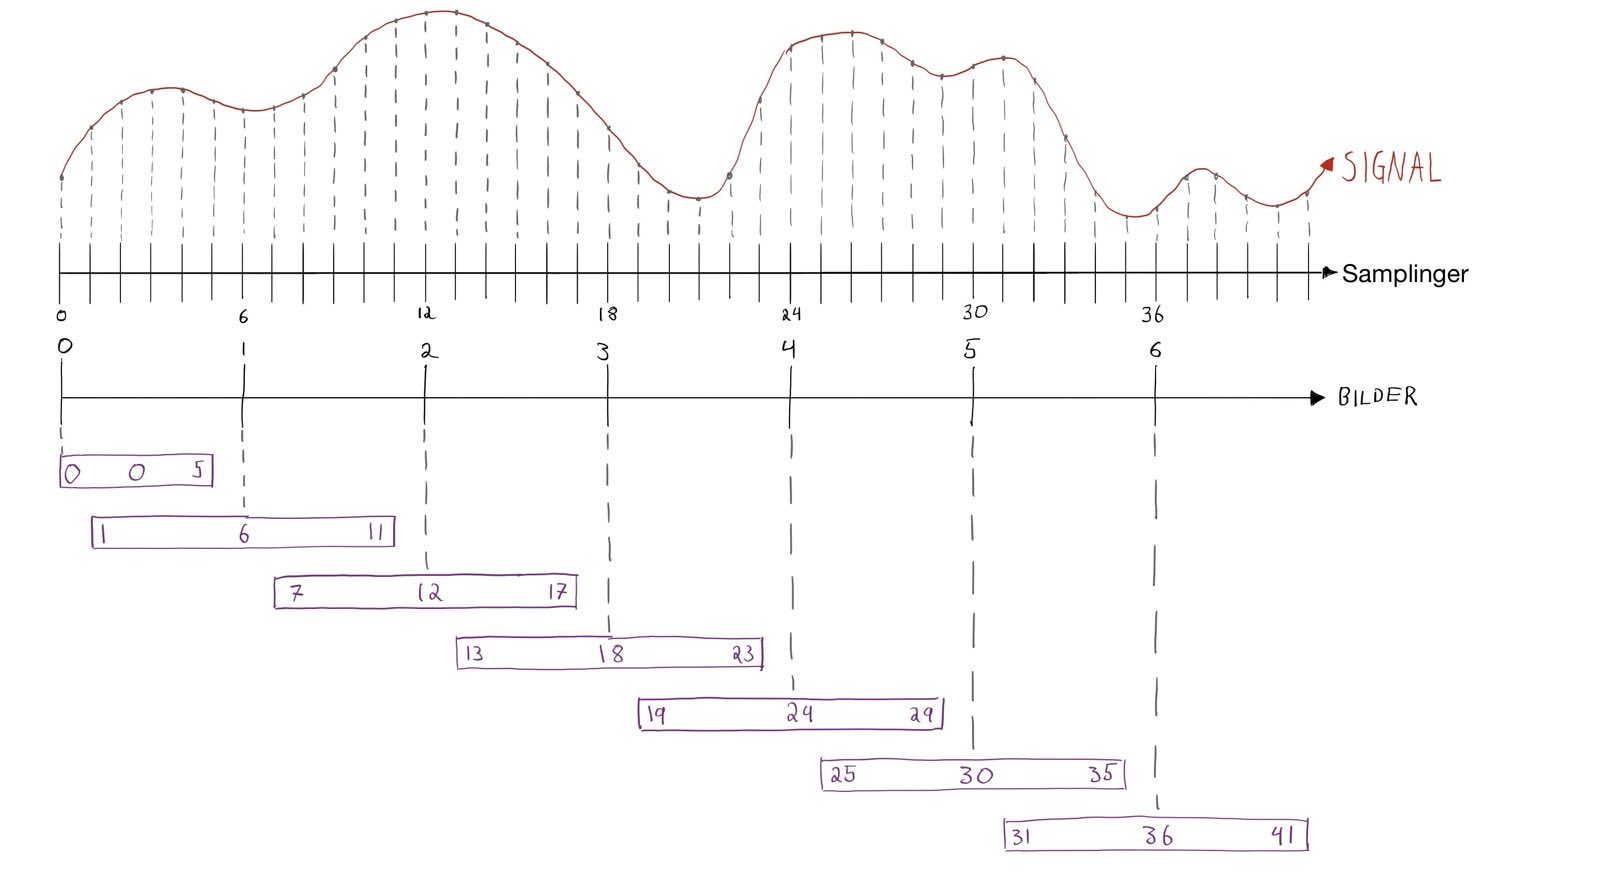
\includegraphics[width=\textwidth]{figurer/samplinger-og-bilder-sammenheng.jpg}
	\caption{Sammenheng mellom sampling og bilder eksempel}
	\label{fig:eksempelSammenhengSamplingOgBilder}
\end{figure}

Figur (\ref{fig:eksempelSammenhengSamplingOgBilder}) viser sammenhengen mellom hvordan programmet håndterer ulike 
fouriertransformasjonsvinduer og ulike bildefrekvenser. Fra eksempelet er det plottet \texttt{41} ulike samplinger, med
en samplingsrate på \texttt{sampleRate = r = 100Hz}. Bildefrekvensen er satt lik \texttt{fps = 16}. Dette gir en samplinger per bilde
verdi på \texttt{spf = 100 / 16 = 6}. Det er satt en tidsluke for hver fouriertransformasjon til \texttt{fft\_t = 0.1s}. Det gir 
antall samplinger per fouriertransformasjon \texttt{N = r * fft\_t = 100Hz * 0.1s = 10}. Betydningen av det
er at for hver sjette sample, renderes det ett nytt bilde. Bildet tar for seg \texttt{N} antall samplinger i fouriertransformasjonen
for bildet. For å få mest mulig overlapp mellom bilder, er blir tar den med fem samplinger før og etter bildet sin
"senter" sampling, som er bestemt av \texttt{n * spf}.

\subsubsection{Plotting og animasjon av bilder}

Ettersom at de høyeste og laveste amplitudeverdiene på ulike lydfiler kan være svært ulik hverandre, starter koden
for plotting ved å finne en maksverdi for amplitude. Det skjer i form av en for-løkke som itererer fra null til 
totale bilder i samplearrayen. Der den for hver iterasjon gjør fouriertransformasjonen, og via funksjonen 
\texttt{np.percentile} finner den gjennomsnittet av $99\%$ av verdiene i den fouriertransformerte arrayen.

Deretter defineres plottingargumentene. Her er navngis aksene, og maksverdi for x og y aksen defineres her. 
Deretter kommer \texttt{animate} funksjonen. Funksjonen tar bildenummer \texttt{i} som argument, og returnerer
\texttt{xf} som x-akse verdier og den fouriertransformerte fo bildet \texttt{y} som grafen. I tilleg blir 
\texttt{infoTekst} returnert, som er boksen i høyre hjørne som viser ulike parametre for hvert bilde. For animasjon
blir funksjonen \texttt{FuncAnimation} brukt. Den tar plottingfigur \texttt{fig}, animasjonsfunksjon \texttt{animate},
initialiseringsfunksjon \texttt{init}, antall bilder \texttt{totalFrames}, tidsintervall mellom hvert bilde 
\texttt{1000/ fps}. For å lagre plotten, brukes funksjonen \texttt{anim.save} brukt. Den lagrer videoen i en 
midlertidig fil, der \texttt{subprocess} biblioteket sin funksjon {sp.run} blir brukt til å kjøre 
\texttt{ffmpeg} programmet for å legge til lyd på programmet. 

\subsection{Spektrogramanalyse i Python}

I dette delkapittelet beskrives koden som brukes for å analysere lydsignalet til sangen 
\textit{Seven Nation Army}, ved å beregne og visualisere et melspektrogram. Programmet 
er skrevet i Python, og benytter pakkene \texttt{librosa}, \texttt{numpy} og \texttt{matplotlib} 
for å lese, behandle og plotte lyddataen. Koden kan hentes her: \parencite{python_mel_spektrogram}

\subsubsection{Melspektrogramfunksjonen}

Først lastes lydfilen inn ved hjelp av funksjonen \texttt{librosa.load}. Denne returnerer 
to verdier: \texttt{y}, som er selve lydsignalet som et array av amplitudeverdier, og 
\texttt{sr}, som er samplingsfrekvensen. Samplingsfrekvensen angir hvor mange ganger per sekund 
den analoge lydbølgen har blitt målt:

\begin{equation*}
    \Delta t = \frac{1}{sr}
\end{equation*}

Signalet \texttt{y} kan dermed beskrives som en tidsdiskret sekvens:

\begin{equation*}
    y = \{x[n]\}_{n=0}^{N-1}
\end{equation*}

hvor \( x[n] \) representerer lydens amplitude ved tidspunkt \( t = n \cdot \Delta t \).

Deretter beregnes et melspektrogram ved hjelp av funksjonen \texttt{librosa.feature.melspectrogram}. 
Denne funksjonen utfører en korttids Fourier-transformasjon (STFT) av signalet:

\begin{equation*}
    X(k,m) = \sum_{n=0}^{N-1} x[n+mH]\, w[n]\, e^{-j2\pi kn/N}
\end{equation*}

Her er \( w[n] \) vindusfunksjonen, \( H \) hop size (forskyvning mellom vinduer), 
\( k \) frekvensbånd og \( m \) tidsvindu.

Etter at STFT er beregnet, konverteres frekvensaksen fra lineær skala til mel-skala, 
som er tilpasset hvordan mennesket oppfatter tonehøyde. Denne skalaen defineres ved:

\begin{equation*}
    \text{mel}(f) = 2595 \cdot \log_{10}\left(1 + \frac{f}{700}\right)
\end{equation*}

Energien i hvert frekvensbånd summeres innenfor et gitt antall mel-bånd for å representere 
lydens spektrale energi på en perceptuell skala.

Videre konverteres energiverdiene i spektrogrammet til desibel (dB) for å fremheve variasjoner 
i lydstyrke. Dette gjøres med:

\begin{equation*}
    S_{\text{dB}} = 10 \cdot \log_{10}\left(\frac{S}{S_{\text{ref}}}\right)
\end{equation*}

hvor \( S_{\text{ref}} = \max(S) \) brukes som referanseverdi slik at den sterkeste 
frekvenskomponenten blir 0 dB.

Til slutt visualiseres melspektrogrammet ved hjelp av funksjonen \texttt{librosa.display.specshow}, 
der x-aksen representerer tid, y-aksen mel-frekvens, og fargene intensitet i dB. Et fargekart viser variasjonen i energi over tid og frekvens, der lysere farger indikerer høyere energi. Figuren viser hvordan frekvensinnholdet i sangen endrer seg over tid, og gir et visuelt grunnlag for videre analyse av rytme og struktur.






\clearpage

\section{Resultater}
% resultater.tex --------------------------------

% Kort kapittelintroduksjon

\subsection{FFT-resultater}
% Presentasjon av resultatene fra Fourier-transformasjonen (hele signalet)
% Beskriv analysens forutsetninger: varighet, samplingsrate og eventuelle filtre

\subsubsection{Spektrumanalyse}
% Presenter resultatet fra FFT-beregningen som figur eller tabell
% Vis det observerte frekvensspekteret og marker de mest fremtredende toppene
% Kommenter kun hvilke frekvenser som forekommer og deres relative styrke
% Unngå forklaring av årsaker – det skal gjøres i diskusjonen

\subsubsection{Harmoniske komponenter}
% Identifiser grunnfrekvens og overtoner i spekteret
% Angi målte verdier i Hz og sammenlign med teoretiske frekvenser uten å vurdere avvik
% Eventuelt bruk tabell for å liste grunnfrekvens + 2–3 harmoniske overtoner

\subsubsection{Amplitude og energifordeling}
% Presenter hvordan signalenergien er fordelt mellom ulike frekvensbånd
% Bruk graf eller tabell for å vise total energi i lav-, mellom- og høyfrekvent område
% Beskriv observasjonene nøytralt uten å forklare årsaker




\subsection{STFT-resultater}
% Resultater fra tids-frekvensanalyse (spektrogram)
% Forklar kort hvilke parametere som ble brukt (vindutype, størrelse, overlapp)

\subsubsection{Spektrogram}
% Vis spektrogrammet som figur med akser for tid og frekvens
% Beskriv de tydelige mønstrene og hvor i tidsaksen de opptrer
% Eksempel: «Tydelige bånd observeres mellom 50–110 Hz gjennom hele klippet»

\subsubsection{Tidsvariasjon og rytmikk}
% Kommenter hvordan spektrogrammet viser variasjoner i tid og rytmiske elementer
% Beskriv observerte mønstre, f.eks. endringer i amplitude eller hyppighet av slag
% Ikke forklar hvorfor variasjonene oppstår – det tas opp i diskusjon.tex





\subsection{Oppsummering}
% Kort oppsummering av hovedfunn fra FFT- og STFT-analysen
% Nevn hvilke frekvensområder og mønstre som ble observert
% Avslutt med en setning som peker frem mot diskusjonsdelen, f.eks.:
% «I neste kapittel drøftes hvordan disse resultatene kan forklares ut fra teori og metodevalg.»


\clearpage

\section{Diskusjon}
% diskusjon.tex

% Innled kort: hensikten med diskusjonen, hvordan resultatene skal vurderes og settes i kontekst

\subsection{Tolkning av resultatene}
Hensikten med dette kapittelet er å drøfte resultatene fra frekvensanalysen, og sette de i sammenheng med teorien om
Fourier-transfomasjoner. Målet er å vurdere hvor godt de praktiske funnene samsvarer med de teoretiske forventningene, samt
belyse metodens styrker, begrensninger og mulig forbedringer.
% Overordnet drøfting av hva resultatene viser og hva de betyr i sammenheng med teorien

\subsubsection{Identifiserte frekvenser}
Resultatene fra frekvensanalysen viser tydelige bånd i området mellom omtrent 55 og 110 Hz, som tilsvarer basslinjen i Seven
Nation Army. Dette stemmer godt overens med forventede verdier for tonene i sangens karakteristiske riff. De lavfrekvente
komponentene dominerer store deler av spektrogrammet, noe som indikerer at bassgitaren har en sentral rolle i lydsignalet.

I tillegg ble flere høyere harmoniske komponenter observert, spesielt i områdene rundt 200-400 Hz og 800-1000 Hz. Disse
representerer overtoner og resonanser som oppstår naturlig når strengen vibrerer, samt bidrag fra andre instrumenter og vokal.
De høyfrekvente toppene som forekommer sporadisk i spektrogrammet, kan tilskrives slagverk og transienter fra trommeslag eller
perkusjon.
% Diskuter hvilke frekvenser som dominerer i analysen
% Forklar hvordan disse stemmer med forventede verdier fra basslinjen
% Kommenter på harmoniske komponenter og hvordan de opptrer i spekteret

\subsubsection{Tidsvariasjon i STFT}
STFT-resultatet gir et tydelig bilde av hvordan frekvensinnholdet i sangen endrer seg over tid. De første sekundene av sangen 
viser stabile lavfrekvente komponenter uten store endringer, noe som samsvarer med introen hvor basslinjen går alene. Etter 
hvert som flere instrumenter legges til, blir spektrogrammet tettere og mer komplekst, med økt energi i mellom- og 
høyfrekvensområdet, noe som antyder at flere instumenter blir med i lydbildet.


Mot slutten av klippet kan man se tydelige variasjoner i amplitude og intensitet, som viser hvordan energien i signalet 
varierer i takt med rytmen og instrumenteringen. STFT-analysen bekrefter dermed at metoden effektivt fanger opp både harmoniske
og rytmiske endringer i musikken.
% Forklar hvordan STFT viser endringer i frekvens over tid
% Diskuter rytmikk, slag og transienter synlig i spektrogrammet
% Knytt dette til hvordan Fourier-transformasjon fanger dynamiske signaler



\subsection{Sammenheng mellom teori og praksis}
% Sammenlign teoretiske prinsipper (DFT, FFT, STFT) med de praktiske resultatene fra analysen

\subsubsection{Forventede vs. observerte mønstre}
De observerte mønstrene i spektrogrammet samsvarer i stor grad med de teoretiske forventningene. Som forventet gir stabile,
periodiske singnaler, for eksempel basslinjen, vedvarende tydlige horisontalbånd, mens raske transienter og slag gir vertikale
mønstre. Dette stemmer overens med teorien om at korte tidsvariasjoner krever bredere frekvensbånd, mens stabile toner gir 
smalere og mer konsentrerte frekvenskomponenter.


Det var en forventning om å kunne identifisere flere intrumenter, men dette er ikke noe som en kunne tydlig observere i 
resultatene. Dette kan skyldes av at mange intrumenter har et lydbilde bestående av mange ulike overtoner og kan dermed være 
vanskelig å skille fra hverandre under analysen.
Små avvik mellom forventet og faktiske resultater kan dermed skyldes av instrumentene eller effekter i lydproduksjonen. Dette 
lager støy i analysen, men en ser likevel et presist bilde av signalets struktur, samt identifisere enkelte instrumenter ved 
STFT og FFT.
% Sammenlign teoretisk forventet spektrum med faktisk FFT-resultat
% Diskuter mulige årsaker til avvik (aliasing, vinduvalg, sampling)

\subsubsection{Effekten av vindustype og parametere}
Valg av vindu har stor betydning for tids- og frekvensoppløsning, samt på resultatet både i leslighet og nøyaktighet. Dermed har det blitt
benyttet Hann-vindu, ettersom denne metoden legger til rette for god balanse mellom tids- og frekvensoppløsningen som passer
til formålet. Samtidig er Hann-vindu god for å redusere spektrallekkasje noe som fører til renere resultater, og er mer 
hensiktsmessig for analyse hvor det er sammensetting av mange u-rene lyder. Et rektangulært vindu ville gitt skarpere 
frekvensoppløsning, men på bekostning av større grad av spektrallekkasje og er derfor ikke like hensiktsmessig.

Hoplengden og FFT-størrelsen påvirker også resultatet. Kortere hoplengde gir bedre tidsoppløsning, men øker beregningstid. 
Større FFT gir bedre frekvenspresisjon, men lavere tidsoppløsning. Dette illustrerer sammenhengen mellom tid og frekvens som er 
beskrevet i teorien. Det ble først valgt FFT størrelse slik at en målte til og med 22050Hz med en Hoplengde på 100ms. Da med slike 
instillinger blir det oppnådd et kompromi hvor en tydelig ser de mest rellevante frekvensenr, men for å få fram resultatene mer tydlig ble det
begrenset et ommrådet til mellom 0Hz og 5000Hz. Ved å gjøre dette blir noe av målingene av overtoner unngått, men får i gjenjeld mye 
klarere resultater på de mest fremtredene frekvensene. 
% Drøft hvordan valg av vindu (Hann, Hamming) påvirket oppløsningen
% Kommenter kompromisset mellom tids- og frekvenspresisjon



\subsection{Begrensninger og feilkilder}
% Drøft svakheter i metode, datainnsamling eller beregning

\subsubsection{Numeriske og tekniske begrensninger}
Selv om FFT og STFT gir gode resultater, finnes det fortsatt numeriske og tekniske begrensninger i løsningen som er blitt har valgt. Flyttallsavrunding og presisjonberegninger i Python kan gi små avvik i beregningene, særlig for lange signaler eller lave amplitude-komponenter. Likevell regnes det med at dette ikke vil være en betydlig feilkilde for hensikten. 
FFT-størrelse og hoplengde påvirker hvordand tid og frekvens prioriteres, og er alltid et kompromiss som kan føre til uskarpheter i beregningene. 
% Beskriv hvordan Python-implementasjon, FFT-størrelse og samplingsrate kan påvirke nøyaktighet

\subsubsection{Usikkerhet i lyddata}
Lydfilens kvalitet og egenskaper kan også påvirke analysen. Komprimering, støy eller romklang under opptak kan indusere støykomponenter som ikke komer fra intrumentene selv. Sterio til mono konvertering kan også føre til tap av faseinformasjon, og instrumenter med mange overtoner kan være vansklige å skille tydlig. Disse faktorene påvirker serlig sekundære detaljer og svake overtoner, men hovedfrekvensene og rytmemønsterene vil fortsatt fremstå tydelig, og vil derfor fortsatt være tilstrekkelig for analysens konklusjoner.
% Diskuter potensielle feilkilder fra selve lydfilen (komprimering, støy, stereo–>mono-konvertering)
% Kommenter hvordan disse kan påvirke analysen



\subsection{Relevans og videre arbeid}
% Sett analysen i en større kontekst og foreslå videre forskning

\subsubsection{Praktisk anvendelse}
Fourier-transformasjoner er et kraftig verktøy som brukes i en rekke reelle systemer. Innen signalbehandling er de essensielle for å analysere og filtrere lydsignaler, som vist i denne analysen av musikk. I musikkteknologi brukes Fourier-analyser for å forstå frekvensspekteret til instrumenter, forbedre lydkvalitet og utvikle effekter som equalizere og reverb. Innen telematikk benyttes Fourier-transformasjoner for å komprimere data, redusere støy og forbedre signaloverføring. Fourier-metoder er også grunnlaget for moderne kommunikasjonsprotokoller, som OFDM brukt i Wi-Fi og 4G/5G-nettverk, og er dermed svært relevante for cyberingeniører og sambandsanalytikere. 
% Forklar hvordan Fourier-transformasjoner brukes i reelle systemer (signalbehandling, musikkteknologi, telematikk)
% Relater gjerne til fagfeltet ditt (cyberingeniør / sambandsanalyse)

\subsubsection{Forslag til videre arbeid}
Denne analysen kan utvides på flere måter for å forbedre nøyaktigheten og anvendeligheten av resultatene. En mulig retning er å implementere Wavelet-transformasjoner, som kan gi bedre tids-frekvensoppløsning for ikke-stasjonære signaler som musikk. Dette kan bidra til å fange opp raske transienter og dynamiske endringer mer effektivt enn STFT. Videre kan en dypere musikkanalyse utforskes, inkludert identifikasjon av individuelle instrumenter og deres bidrag til det samlede lydbildet. Dette kan innebære bruk av maskinlæringsteknikker for å klassifisere og separere lydkilder basert på deres frekvenskarakteristikker, ettersom det kan vise seg å være problematisk å gjøre dette med høy nøyaktighet uten hjelpeverktøy. 
% Foreslå utvidelser: f.eks. Wavelet-transformasjon, dypere musikkanalyse, sanntidsimplementasjon
% Reflekter kort over hvordan prosjektet kan forbedres

% Kort avsluttende avsnitt uten undertittel:
% Oppsummer hovedpoengene fra diskusjonen og legg opp til konklusjonskapittelet



\clearpage

\section{Konklusjon}
% konklusjon.tex

% Kort kapittelintroduksjon
% Kort oppsummering av hva prosjektet har undersøkt og oppnådd


\subsection{Oppsummering av funn}
% Oppsummer de viktigste resultatene fra analysen
% Nevn hovedfrekvenser, mønstre og eventuelle sammenhenger observert i FFT/STFT
% Forklar hvordan funnene støtter teorien om Fourier-transformasjonens anvendelse



\subsection{Vurdering av metode}
% Evaluer hvor godt metodene (DFT, FFT, STFT) fungerte for formålet
% Kommenter styrker, begrensninger og nøyaktighet i analysen
% Kort refleksjon over valg av parametere (vindu, samplingrate osv.)




\subsection{Forbedringsmuligheter og videre arbeid}
% Foreslå hvordan analysen kan forbedres i fremtidig arbeid
% F.eks. bruk av Wavelet-transformasjon, høyere oppløsning, lengre datasett eller flere signaler
% Eventuelt vurder praktiske anvendelser av metoden innen lydanalyse eller kommunikasjon




\subsection{Avsluttende refleksjon}
% Kort avslutning som binder sammen mål, metode og resultat
% Fremhev hva prosjektet viser om Fourier-transformasjonens relevans og anvendbarhet


\clearpage

\printbibliography

\clearpage

\appendix
\section*{Vedlegg}
\subsection*{Kode for spektrumanalyse}
\label{app:kode_spektrumanalyse}
Kode for spektrumanalyse kan hentes her: \url{}

\subsection*{Video av spektrumanalyse for hele sangen}
\label{app:video_spektrumanalyse}
Videoen kan sees her: \url{}

\subsection*{Kode for spektogramgenerering}
\label{app:kode_spektogramgenerering}
Kode for spektrumanalyse kan hentes her: \url{}



\end{document}
